\documentclass[11pt]{article}
\usepackage[letterpaper,margin=1in]{geometry}
\usepackage[T1]{fontenc}
\usepackage{times}
%%%%% NEW MATH DEFINITIONS %%%%%

\usepackage{amsmath,amsfonts,bm}

% Mark sections of captions for referring to divisions of figures
\newcommand{\figleft}{{\em (Left)}}
\newcommand{\figcenter}{{\em (Center)}}
\newcommand{\figright}{{\em (Right)}}
\newcommand{\figtop}{{\em (Top)}}
\newcommand{\figbottom}{{\em (Bottom)}}
\newcommand{\captiona}{{\em (a)}}
\newcommand{\captionb}{{\em (b)}}
\newcommand{\captionc}{{\em (c)}}
\newcommand{\captiond}{{\em (d)}}

% Highlight a newly defined term
\newcommand{\newterm}[1]{{\bf #1}}


% Figure reference, lower-case.
\def\figref#1{figure~\ref{#1}}
% Figure reference, capital. For start of sentence
\def\Figref#1{Figure~\ref{#1}}
\def\twofigref#1#2{figures \ref{#1} and \ref{#2}}
\def\quadfigref#1#2#3#4{figures \ref{#1}, \ref{#2}, \ref{#3} and \ref{#4}}
% Section reference, lower-case.
\def\secref#1{section~\ref{#1}}
% Section reference, capital.
\def\Secref#1{Section~\ref{#1}}
% Reference to two sections.
\def\twosecrefs#1#2{sections \ref{#1} and \ref{#2}}
% Reference to three sections.
\def\secrefs#1#2#3{sections \ref{#1}, \ref{#2} and \ref{#3}}
% Reference to an equation, lower-case.
\def\eqref#1{equation~\ref{#1}}
% Reference to an equation, upper case
\def\Eqref#1{Equation~\ref{#1}}
% A raw reference to an equation---avoid using if possible
\def\plaineqref#1{\ref{#1}}
% Reference to a chapter, lower-case.
\def\chapref#1{chapter~\ref{#1}}
% Reference to an equation, upper case.
\def\Chapref#1{Chapter~\ref{#1}}
% Reference to a range of chapters
\def\rangechapref#1#2{chapters\ref{#1}--\ref{#2}}
% Reference to an algorithm, lower-case.
\def\algref#1{algorithm~\ref{#1}}
% Reference to an algorithm, upper case.
\def\Algref#1{Algorithm~\ref{#1}}
\def\twoalgref#1#2{algorithms \ref{#1} and \ref{#2}}
\def\Twoalgref#1#2{Algorithms \ref{#1} and \ref{#2}}
% Reference to a part, lower case
\def\partref#1{part~\ref{#1}}
% Reference to a part, upper case
\def\Partref#1{Part~\ref{#1}}
\def\twopartref#1#2{parts \ref{#1} and \ref{#2}}

\def\ceil#1{\lceil #1 \rceil}
\def\floor#1{\lfloor #1 \rfloor}
\def\1{\bm{1}}
\newcommand{\train}{\mathcal{D}}
\newcommand{\valid}{\mathcal{D_{\mathrm{valid}}}}
\newcommand{\test}{\mathcal{D_{\mathrm{test}}}}

\def\eps{{\epsilon}}


% Random variables
\def\reta{{\textnormal{$\eta$}}}
\def\ra{{\textnormal{a}}}
\def\rb{{\textnormal{b}}}
\def\rc{{\textnormal{c}}}
\def\rd{{\textnormal{d}}}
\def\re{{\textnormal{e}}}
\def\rf{{\textnormal{f}}}
\def\rg{{\textnormal{g}}}
\def\rh{{\textnormal{h}}}
\def\ri{{\textnormal{i}}}
\def\rj{{\textnormal{j}}}
\def\rk{{\textnormal{k}}}
\def\rl{{\textnormal{l}}}
% rm is already a command, just don't name any random variables m
\def\rn{{\textnormal{n}}}
\def\ro{{\textnormal{o}}}
\def\rp{{\textnormal{p}}}
\def\rq{{\textnormal{q}}}
\def\rr{{\textnormal{r}}}
\def\rs{{\textnormal{s}}}
\def\rt{{\textnormal{t}}}
\def\ru{{\textnormal{u}}}
\def\rv{{\textnormal{v}}}
\def\rw{{\textnormal{w}}}
\def\rx{{\textnormal{x}}}
\def\ry{{\textnormal{y}}}
\def\rz{{\textnormal{z}}}

% Random vectors
\def\rvepsilon{{\mathbf{\epsilon}}}
\def\rvtheta{{\mathbf{\theta}}}
\def\rva{{\mathbf{a}}}
\def\rvb{{\mathbf{b}}}
\def\rvc{{\mathbf{c}}}
\def\rvd{{\mathbf{d}}}
\def\rve{{\mathbf{e}}}
\def\rvf{{\mathbf{f}}}
\def\rvg{{\mathbf{g}}}
\def\rvh{{\mathbf{h}}}
\def\rvu{{\mathbf{i}}}
\def\rvj{{\mathbf{j}}}
\def\rvk{{\mathbf{k}}}
\def\rvl{{\mathbf{l}}}
\def\rvm{{\mathbf{m}}}
\def\rvn{{\mathbf{n}}}
\def\rvo{{\mathbf{o}}}
\def\rvp{{\mathbf{p}}}
\def\rvq{{\mathbf{q}}}
\def\rvr{{\mathbf{r}}}
\def\rvs{{\mathbf{s}}}
\def\rvt{{\mathbf{t}}}
\def\rvu{{\mathbf{u}}}
\def\rvv{{\mathbf{v}}}
\def\rvw{{\mathbf{w}}}
\def\rvx{{\mathbf{x}}}
\def\rvy{{\mathbf{y}}}
\def\rvz{{\mathbf{z}}}

% Elements of random vectors
\def\erva{{\textnormal{a}}}
\def\ervb{{\textnormal{b}}}
\def\ervc{{\textnormal{c}}}
\def\ervd{{\textnormal{d}}}
\def\erve{{\textnormal{e}}}
\def\ervf{{\textnormal{f}}}
\def\ervg{{\textnormal{g}}}
\def\ervh{{\textnormal{h}}}
\def\ervi{{\textnormal{i}}}
\def\ervj{{\textnormal{j}}}
\def\ervk{{\textnormal{k}}}
\def\ervl{{\textnormal{l}}}
\def\ervm{{\textnormal{m}}}
\def\ervn{{\textnormal{n}}}
\def\ervo{{\textnormal{o}}}
\def\ervp{{\textnormal{p}}}
\def\ervq{{\textnormal{q}}}
\def\ervr{{\textnormal{r}}}
\def\ervs{{\textnormal{s}}}
\def\ervt{{\textnormal{t}}}
\def\ervu{{\textnormal{u}}}
\def\ervv{{\textnormal{v}}}
\def\ervw{{\textnormal{w}}}
\def\ervx{{\textnormal{x}}}
\def\ervy{{\textnormal{y}}}
\def\ervz{{\textnormal{z}}}

% Random matrices
\def\rmA{{\mathbf{A}}}
\def\rmB{{\mathbf{B}}}
\def\rmC{{\mathbf{C}}}
\def\rmD{{\mathbf{D}}}
\def\rmE{{\mathbf{E}}}
\def\rmF{{\mathbf{F}}}
\def\rmG{{\mathbf{G}}}
\def\rmH{{\mathbf{H}}}
\def\rmI{{\mathbf{I}}}
\def\rmJ{{\mathbf{J}}}
\def\rmK{{\mathbf{K}}}
\def\rmL{{\mathbf{L}}}
\def\rmM{{\mathbf{M}}}
\def\rmN{{\mathbf{N}}}
\def\rmO{{\mathbf{O}}}
\def\rmP{{\mathbf{P}}}
\def\rmQ{{\mathbf{Q}}}
\def\rmR{{\mathbf{R}}}
\def\rmS{{\mathbf{S}}}
\def\rmT{{\mathbf{T}}}
\def\rmU{{\mathbf{U}}}
\def\rmV{{\mathbf{V}}}
\def\rmW{{\mathbf{W}}}
\def\rmX{{\mathbf{X}}}
\def\rmY{{\mathbf{Y}}}
\def\rmZ{{\mathbf{Z}}}

% Elements of random matrices
\def\ermA{{\textnormal{A}}}
\def\ermB{{\textnormal{B}}}
\def\ermC{{\textnormal{C}}}
\def\ermD{{\textnormal{D}}}
\def\ermE{{\textnormal{E}}}
\def\ermF{{\textnormal{F}}}
\def\ermG{{\textnormal{G}}}
\def\ermH{{\textnormal{H}}}
\def\ermI{{\textnormal{I}}}
\def\ermJ{{\textnormal{J}}}
\def\ermK{{\textnormal{K}}}
\def\ermL{{\textnormal{L}}}
\def\ermM{{\textnormal{M}}}
\def\ermN{{\textnormal{N}}}
\def\ermO{{\textnormal{O}}}
\def\ermP{{\textnormal{P}}}
\def\ermQ{{\textnormal{Q}}}
\def\ermR{{\textnormal{R}}}
\def\ermS{{\textnormal{S}}}
\def\ermT{{\textnormal{T}}}
\def\ermU{{\textnormal{U}}}
\def\ermV{{\textnormal{V}}}
\def\ermW{{\textnormal{W}}}
\def\ermX{{\textnormal{X}}}
\def\ermY{{\textnormal{Y}}}
\def\ermZ{{\textnormal{Z}}}

% Vectors
\def\vzero{{\bm{0}}}
\def\vone{{\bm{1}}}
\def\vmu{{\bm{\mu}}}
\def\vtheta{{\bm{\theta}}}
\def\va{{\bm{a}}}
\def\vb{{\bm{b}}}
\def\vc{{\bm{c}}}
\def\vd{{\bm{d}}}
\def\ve{{\bm{e}}}
\def\vf{{\bm{f}}}
\def\vg{{\bm{g}}}
\def\vh{{\bm{h}}}
\def\vi{{\bm{i}}}
\def\vj{{\bm{j}}}
\def\vk{{\bm{k}}}
\def\vl{{\bm{l}}}
\def\vm{{\bm{m}}}
\def\vn{{\bm{n}}}
\def\vo{{\bm{o}}}
\def\vp{{\bm{p}}}
\def\vq{{\bm{q}}}
\def\vr{{\bm{r}}}
\def\vs{{\bm{s}}}
\def\vt{{\bm{t}}}
\def\vu{{\bm{u}}}
\def\vv{{\bm{v}}}
\def\vw{{\bm{w}}}
\def\vx{{\bm{x}}}
\def\vy{{\bm{y}}}
\def\vz{{\bm{z}}}

% Elements of vectors
\def\evalpha{{\alpha}}
\def\evbeta{{\beta}}
\def\evepsilon{{\epsilon}}
\def\evlambda{{\lambda}}
\def\evomega{{\omega}}
\def\evmu{{\mu}}
\def\evpsi{{\psi}}
\def\evsigma{{\sigma}}
\def\evtheta{{\theta}}
\def\eva{{a}}
\def\evb{{b}}
\def\evc{{c}}
\def\evd{{d}}
\def\eve{{e}}
\def\evf{{f}}
\def\evg{{g}}
\def\evh{{h}}
\def\evi{{i}}
\def\evj{{j}}
\def\evk{{k}}
\def\evl{{l}}
\def\evm{{m}}
\def\evn{{n}}
\def\evo{{o}}
\def\evp{{p}}
\def\evq{{q}}
\def\evr{{r}}
\def\evs{{s}}
\def\evt{{t}}
\def\evu{{u}}
\def\evv{{v}}
\def\evw{{w}}
\def\evx{{x}}
\def\evy{{y}}
\def\evz{{z}}

% Matrix
\def\mA{{\bm{A}}}
\def\mB{{\bm{B}}}
\def\mC{{\bm{C}}}
\def\mD{{\bm{D}}}
\def\mE{{\bm{E}}}
\def\mF{{\bm{F}}}
\def\mG{{\bm{G}}}
\def\mH{{\bm{H}}}
\def\mI{{\bm{I}}}
\def\mJ{{\bm{J}}}
\def\mK{{\bm{K}}}
\def\mL{{\bm{L}}}
\def\mM{{\bm{M}}}
\def\mN{{\bm{N}}}
\def\mO{{\bm{O}}}
\def\mP{{\bm{P}}}
\def\mQ{{\bm{Q}}}
\def\mR{{\bm{R}}}
\def\mS{{\bm{S}}}
\def\mT{{\bm{T}}}
\def\mU{{\bm{U}}}
\def\mV{{\bm{V}}}
\def\mW{{\bm{W}}}
\def\mX{{\bm{X}}}
\def\mY{{\bm{Y}}}
\def\mZ{{\bm{Z}}}
\def\mBeta{{\bm{\beta}}}
\def\mPhi{{\bm{\Phi}}}
\def\mLambda{{\bm{\Lambda}}}
\def\mSigma{{\bm{\Sigma}}}

% Tensor
\DeclareMathAlphabet{\mathsfit}{\encodingdefault}{\sfdefault}{m}{sl}
\SetMathAlphabet{\mathsfit}{bold}{\encodingdefault}{\sfdefault}{bx}{n}
\newcommand{\tens}[1]{\bm{\mathsfit{#1}}}
\def\tA{{\tens{A}}}
\def\tB{{\tens{B}}}
\def\tC{{\tens{C}}}
\def\tD{{\tens{D}}}
\def\tE{{\tens{E}}}
\def\tF{{\tens{F}}}
\def\tG{{\tens{G}}}
\def\tH{{\tens{H}}}
\def\tI{{\tens{I}}}
\def\tJ{{\tens{J}}}
\def\tK{{\tens{K}}}
\def\tL{{\tens{L}}}
\def\tM{{\tens{M}}}
\def\tN{{\tens{N}}}
\def\tO{{\tens{O}}}
\def\tP{{\tens{P}}}
\def\tQ{{\tens{Q}}}
\def\tR{{\tens{R}}}
\def\tS{{\tens{S}}}
\def\tT{{\tens{T}}}
\def\tU{{\tens{U}}}
\def\tV{{\tens{V}}}
\def\tW{{\tens{W}}}
\def\tX{{\tens{X}}}
\def\tY{{\tens{Y}}}
\def\tZ{{\tens{Z}}}


% Graph
\def\gA{{\mathcal{A}}}
\def\gB{{\mathcal{B}}}
\def\gC{{\mathcal{C}}}
\def\gD{{\mathcal{D}}}
\def\gE{{\mathcal{E}}}
\def\gF{{\mathcal{F}}}
\def\gG{{\mathcal{G}}}
\def\gH{{\mathcal{H}}}
\def\gI{{\mathcal{I}}}
\def\gJ{{\mathcal{J}}}
\def\gK{{\mathcal{K}}}
\def\gL{{\mathcal{L}}}
\def\gM{{\mathcal{M}}}
\def\gN{{\mathcal{N}}}
\def\gO{{\mathcal{O}}}
\def\gP{{\mathcal{P}}}
\def\gQ{{\mathcal{Q}}}
\def\gR{{\mathcal{R}}}
\def\gS{{\mathcal{S}}}
\def\gT{{\mathcal{T}}}
\def\gU{{\mathcal{U}}}
\def\gV{{\mathcal{V}}}
\def\gW{{\mathcal{W}}}
\def\gX{{\mathcal{X}}}
\def\gY{{\mathcal{Y}}}
\def\gZ{{\mathcal{Z}}}

% Sets
\def\sA{{\mathbb{A}}}
\def\sB{{\mathbb{B}}}
\def\sC{{\mathbb{C}}}
\def\sD{{\mathbb{D}}}
% Don't use a set called E, because this would be the same as our symbol
% for expectation.
\def\sF{{\mathbb{F}}}
\def\sG{{\mathbb{G}}}
\def\sH{{\mathbb{H}}}
\def\sI{{\mathbb{I}}}
\def\sJ{{\mathbb{J}}}
\def\sK{{\mathbb{K}}}
\def\sL{{\mathbb{L}}}
\def\sM{{\mathbb{M}}}
\def\sN{{\mathbb{N}}}
\def\sO{{\mathbb{O}}}
\def\sP{{\mathbb{P}}}
\def\sQ{{\mathbb{Q}}}
\def\sR{{\mathbb{R}}}
\def\sS{{\mathbb{S}}}
\def\sT{{\mathbb{T}}}
\def\sU{{\mathbb{U}}}
\def\sV{{\mathbb{V}}}
\def\sW{{\mathbb{W}}}
\def\sX{{\mathbb{X}}}
\def\sY{{\mathbb{Y}}}
\def\sZ{{\mathbb{Z}}}

% Entries of a matrix
\def\emLambda{{\Lambda}}
\def\emA{{A}}
\def\emB{{B}}
\def\emC{{C}}
\def\emD{{D}}
\def\emE{{E}}
\def\emF{{F}}
\def\emG{{G}}
\def\emH{{H}}
\def\emI{{I}}
\def\emJ{{J}}
\def\emK{{K}}
\def\emL{{L}}
\def\emM{{M}}
\def\emN{{N}}
\def\emO{{O}}
\def\emP{{P}}
\def\emQ{{Q}}
\def\emR{{R}}
\def\emS{{S}}
\def\emT{{T}}
\def\emU{{U}}
\def\emV{{V}}
\def\emW{{W}}
\def\emX{{X}}
\def\emY{{Y}}
\def\emZ{{Z}}
\def\emSigma{{\Sigma}}

% entries of a tensor
% Same font as tensor, without \bm wrapper
\newcommand{\etens}[1]{\mathsfit{#1}}
\def\etLambda{{\etens{\Lambda}}}
\def\etA{{\etens{A}}}
\def\etB{{\etens{B}}}
\def\etC{{\etens{C}}}
\def\etD{{\etens{D}}}
\def\etE{{\etens{E}}}
\def\etF{{\etens{F}}}
\def\etG{{\etens{G}}}
\def\etH{{\etens{H}}}
\def\etI{{\etens{I}}}
\def\etJ{{\etens{J}}}
\def\etK{{\etens{K}}}
\def\etL{{\etens{L}}}
\def\etM{{\etens{M}}}
\def\etN{{\etens{N}}}
\def\etO{{\etens{O}}}
\def\etP{{\etens{P}}}
\def\etQ{{\etens{Q}}}
\def\etR{{\etens{R}}}
\def\etS{{\etens{S}}}
\def\etT{{\etens{T}}}
\def\etU{{\etens{U}}}
\def\etV{{\etens{V}}}
\def\etW{{\etens{W}}}
\def\etX{{\etens{X}}}
\def\etY{{\etens{Y}}}
\def\etZ{{\etens{Z}}}

% The true underlying data generating distribution
\newcommand{\pdata}{p_{\rm{data}}}
% The empirical distribution defined by the training set
\newcommand{\ptrain}{\hat{p}_{\rm{data}}}
\newcommand{\Ptrain}{\hat{P}_{\rm{data}}}
% The model distribution
\newcommand{\pmodel}{p_{\rm{model}}}
\newcommand{\Pmodel}{P_{\rm{model}}}
\newcommand{\ptildemodel}{\tilde{p}_{\rm{model}}}
% Stochastic autoencoder distributions
\newcommand{\pencode}{p_{\rm{encoder}}}
\newcommand{\pdecode}{p_{\rm{decoder}}}
\newcommand{\precons}{p_{\rm{reconstruct}}}

\newcommand{\laplace}{\mathrm{Laplace}} % Laplace distribution

\newcommand{\E}{\mathbb{E}}
\newcommand{\Ls}{\mathcal{L}}
\newcommand{\R}{\mathbb{R}}
\newcommand{\emp}{\tilde{p}}
\newcommand{\lr}{\alpha}
\newcommand{\reg}{\lambda}
\newcommand{\rect}{\mathrm{rectifier}}
\newcommand{\softmax}{\mathrm{softmax}}
\newcommand{\sigmoid}{\sigma}
\newcommand{\softplus}{\zeta}
\newcommand{\KL}{D_{\mathrm{KL}}}
\newcommand{\Var}{\mathrm{Var}}
\newcommand{\standarderror}{\mathrm{SE}}
\newcommand{\Cov}{\mathrm{Cov}}
% Wolfram Mathworld says $L^2$ is for function spaces and $\ell^2$ is for vectors
% But then they seem to use $L^2$ for vectors throughout the site, and so does
% wikipedia.
\newcommand{\normlzero}{L^0}
\newcommand{\normlone}{L^1}
\newcommand{\normltwo}{L^2}
\newcommand{\normlp}{L^p}
\newcommand{\normmax}{L^\infty}

\newcommand{\parents}{Pa} % See usage in notation.tex. Chosen to match Daphne's book.

\DeclareMathOperator*{\argmax}{arg\,max}
\DeclareMathOperator*{\argmin}{arg\,min}

\DeclareMathOperator{\sign}{sign}
\DeclareMathOperator{\Tr}{Tr}
\let\ab\allowbreak

\usepackage[round]{natbib}
\usepackage{xcolor}
\usepackage[colorlinks=true,linkcolor=blue!60!black,citecolor=blue!60!black,urlcolor=blue!60!black]{hyperref}
\usepackage{url}
\usepackage{booktabs}
\usepackage{graphicx}
\usepackage{amsmath,amssymb}
\usepackage{xspace}
\usepackage{fancyhdr}
\usepackage{titlesec}
\titlespacing*{\section}{0pt}{1.4ex plus .5ex minus .2ex}{0.8ex}
\titlespacing*{\subsection}{0pt}{1.1ex plus .4ex minus .2ex}{0.6ex}
\renewcommand{\topfraction}{0.95}
\renewcommand{\textfraction}{0.05}
\setlength{\emergencystretch}{3em}
\newcommand{\ie}{i.e.,\xspace}
\newcommand{\eg}{e.g.,\xspace}
\newcommand{\SCALESENTENCE}{Across further pairs the picture is mixed: real-text bridges come close to the receiver's own states for a second Pythia pair and for GPT-2 into Pythia, but not when a smaller sender feeds a much stronger receiver (Pythia 160M into 410M, GPT-2 into Qwen2.5), and reach only 28\% for OPT into GPT-2 despite a shared tokenizer. The content contrast alone can mislead: with a stronger sender it rises for the LLM-text bridge while no improvement in the receiver's predictions is detected. A second LLM's text also works, at an equal number of characters LLM-written text gives 92--95\% of real text's content but about 75\% of its net gain, and real- and LLM-text bridges fitted on encyclopedic text keep 73--81\% of each domain's own reference content on long movie reviews but about 30\% on source code, where their net effects diverge.}
\newcommand{\SCALECONTRIB}{Beyond the main pair, results are mixed: LLM-text bridges keep 69--72\% of the reference's net gain in four of the six reported model pairs, but cross-family bridging ranges from as good as within Pythia to poor, and the content contrast alone can mislead (\S\ref{sec:scale}).}
\newcommand{\SCALEDISCUSSION}{The generalisation experiments add two cautions. First, report net gain next to any matched-versus-swapped contrast: with a stronger sender the LLM-text bridge's contrast rose while no improvement in the receiver's predictions was detected. Second, synthetic text is not interchangeable: a second LLM's encyclopedia text worked somewhat less well, fiction much less, and an equal number of characters of real text still gave about a third more net gain. Domain matters as well: relative to each domain's own reference, real- and LLM-text bridges fitted on encyclopedic text kept 73--81\% of the content on long reviews but about 30\% on code, and on code the ranking of probe sources by net gain changed.}
\newcommand{\SCALESEEDS}{Larger and cross-family pairs use two or three fits, the capacity ablation one.}
\newcommand{\CEILLONE}{34.3}
\newcommand{\CEILLSIX}{26.2}
\newcommand{\CEILFULL}{37.1}
\newcommand{\CEILNONE}{24.0}
\newcommand{\FREESWEEP}{Selection does not need corpus text either (a check we ran after the main experiments): fitting on the 24 LLM-written articles of the main experiments and validating on the other 40 LLM-written articles selects the same pair ($L_A=2$, $L_B=1$; validation CE 3.531, next best 3.593), so the LLM-text pipeline below uses no real corpus text for bridge fitting or layer selection.}

\newcommand{\XFAMILYINTRO}{and, to test generality, pairs from different families with different tokenizers (GPT-2, OPT and Qwen2.5).}
\newcommand{\SWEEPAPPENDIX}{\paragraph{Selection without corpus text.} The same sweep with bridges fitted on the 24 LLM-written articles used in the main experiments and scored on 256 windows from the other 40 LLM-written articles (no corpus text at any stage):
\begin{center}\small
\begin{tabular}{lcccccc}
\toprule
$L_A$ & 1 & 2 & 3 & 4 & 5 & 6 \\
\midrule
$L_B=1$ & 3.804 & \textbf{3.531} & 3.623 & 3.699 & 3.633 & 4.084 \\
$L_B=2$ & 3.633 & 3.593 & 3.636 & 3.692 & 3.738 & 4.075 \\
\bottomrule
\end{tabular}
\end{center}
Receiver-state reference on these windows: 3.424 ($L_B=1$), 3.457 ($L_B=2$). It selects the same pair as the WikiText validation sweep.}
\newcommand{\XFAMILYLIMIT}{We test three Pythia sizes (up to 410M) and three cross-family pairs (up to 0.5B); results differ widely between pairs, the cross-family runs use two seeds and a restricted layer search, and all models are small.}
\newcommand{\SCALEREVERSE}{}% superseded; the reversed pair is discussed in sec_general.tex
\newcommand{\XFAMILYRESULTS}{For pairs with different tokenizers, windows are defined in the receiver's tokenisation and the sender reads the same prefix text in its own (Appendix~\ref{app:general}); only the communication objective is used, since it needs no token alignment. From GPT-2 (layer 4) into pythia-160m (layer 1), on the main pair's test windows, the real-text bridge again comes close to the receiver's own states (content 1.02 [0.98, 1.05], net 1.00 [0.97, 1.03]), LLM-written text reaches 0.87 and 0.70, self-samples 0.70 and 0.54, and the weight-only map, fitted on 36{,}938 shared token strings, 0.02 in content. Under our protocol and for this pair, models from different organisations, trained on different corpora with different tokenizers, are bridged about as well as two Pythia models. \XQWENOPT}
\newcommand{\XQWENOPT}{From GPT-2 into Qwen2.5-0.5B, a much stronger receiver whose own layer-1 states already give 96\% of the content of text, no bridge comes close: content ratios 0.50 [0.25, 0.76] for real text and 0.57 [0.46, 0.67] for LLM-written text, with very different seeds (real text 0.75 and 0.26). This pair is handicapped by our protocol: the sender reads only the last 90 tokens of its re-tokenised prefix ($P_A=90$, set by digit-heavy prefixes that Qwen splits into single-digit tokens), on average 74\% of the prefix, while the reference uses all of it. Six hundred steps may also be too few for a receiver with a 152k-token vocabulary. Two seeds do not let us separate these causes, so this pair shows only that our protocol does not reach a much stronger receiver's own states. \XOPT}
\newcommand{\TEXTSOURCES}{Is the LLM-written result specific to one model or one batch of text? We generated two further corpora on 24 other topic areas, truncated to 371k characters each: encyclopedia articles from a different LLM (GPT, same prompt) and fiction with narration and dialogue from the same LLM. With two fitting seeds each, content ratios are 0.77 [0.74, 0.81] for the first LLM's encyclopedia text, 0.69 [0.66, 0.72] for the second LLM's and 0.55 [0.52, 0.58] for fiction (net ratios 0.55, 0.52 and 0.31; pairwise content differences 0.08 [0.06, 0.11], 0.23 [0.19, 0.28] and 0.15 [0.12, 0.18] nats). A second LLM's encyclopedia text also yields a working bridge, and these encyclopedia corpora beat this fiction corpus. The comparison does not separate author from register: the corpora differ in token count (72k to 96k tokens for the same characters), in which topics survive truncation (20 to 24), and each is a single generated sample; we lack the GPT-fiction cell. \TEXTSCALE}
\newcommand{\CAPACITY}{Restricting the main pair's bridge to rank 16 or 64 (one seed) leaves content ratios of 0.22 and 0.61 for real text and 0.34 and 0.55 for LLM-written text, against 0.94 and 0.80 for the full-rank bridge of the same seed; real-text low-rank bridges keep a much larger share of net gain (0.51 and 0.76) than of content, i.e.\ a large generic part. Adding an MLP branch (width 2048) moves the same-seed real-text bridge from 0.94 to 0.97 in content and 0.97 to 1.00 net, and the LLM-text bridge from 0.80 to 0.86 and 0.72 to 0.78. With one seed and capacity, parameterisation and optimisation varied together, we read these as descriptive: relative to the same-seed full-rank bridge, rank 16 keeps 23\% (real text) and 43\% (LLM text) of the content and rank 64 keeps 64\% and 69\%, and extra capacity helps the LLM-text bridge somewhat more than the real-text one.}
\newcommand{\TEXTSCALE}{Finally, we compared real and LLM-written text at equal numbers of characters, taking the first 383k or 1.03M characters of each corpus (two seeds; real text taken from the start of the ordered WikiText training split, unlike the main bridge, which samples the full 8.8M-character pool). Real text reaches content ratios 0.87 [0.82, 0.93] and 0.91 [0.88, 0.93] and net ratios 0.92 and 0.96; LLM-written text reaches 0.80 [0.78, 0.83] and 0.86 [0.81, 0.90] in content but only 0.69 and 0.73 net. On content, LLM-written text thus gives 92\% and 95\% of what the same number of characters of real text gives; on net gain, 75\% and 76\%. These are fixed corpora rather than random subsets, so the experiment does not attribute the main gap to quantity.}
\newcommand{\XOPT}{From OPT-125M into GPT-2, two models of similar size that even share a tokenizer, bridges deliver only 0.28 [0.26, 0.30] of the receiver's own states' content with real text and 0.28 [0.25, 0.31] with LLM-written text, consistently across seeds; the real-text bridge also has a large positive generic part (about 36\% of its net gain). Its layer search covered only $L_A\in\{1,2,4\}$, and with GPT-2's absolute position embeddings the generic and net parts may include a position-offset effect (Appendix~\ref{app:general}), while matched and donor messages are compared at identical position offsets. Cross-family bridging is therefore not uniformly easy: it succeeded for one pair, partly for one and poorly for one.}


\pagestyle{fancy}
\fancyhf{}
\fancyhead[L]{\small\textsc{Preprint}}
\fancyhead[R]{\small Content or Context? Latent Communication Between Language Models}
\fancyfoot[C]{\thepage}
\renewcommand{\headrulewidth}{0.4pt}

\title{\textbf{Content or Context? Measuring Latent Communication\\ Between Language Models, with Bridges Fitted\\ on LLM-Written Text}}
\author{Zhaohe Dong\\[2pt]
University of Cambridge\\[2pt]
\texttt{dongzhaohe321418@outlook.com}}
\date{November 2026}

\begin{document}
\maketitle
\thispagestyle{fancy}

\begin{abstract}
Language models can be wired together through their hidden states, and several systems report that such latent channels help. Two questions are rarely separated: how much of a message's benefit is content the receiver lacks, and does building the channel require real text from the models' training distribution? We study both with an information-asymmetric protocol: a sender reads a prefix the receiver never sees, the receiver gets the sender's hidden states through a learned bridge, and donor messages from other windows decompose the receiver's gain into generic, article-level and window-specific parts. The choice of donor is decisive: swapping messages within a batch, where most donors come from the same document, attributes 54\% of a bridge's benefit to generic context; with donors from other documents the generic part is 6\%. Between independently pretrained Pythia models, a linear bridge fitted on real text gives the receiver about the same content gain as the receiver's own prefix states injected the same way (ratio 0.99 [0.94, 1.03]). A bridge fitted only on encyclopedia-style text written by an LLM with no corpus access, with layer selection also done on such text, reaches 82\% [79, 85] of that reference's content gain; bridges fitted on the models' own samples reach 44--59\%, and a weight-only least-squares map 2\%. In the main WikiText experiment, bridges fitted with the tested synthetic-text recipes leave the receiver worse off on average than no message when the message comes from a different document, unlike the real-text bridge. \SCALESENTENCE
\end{abstract}
\begin{center}\small Code, results and fitted bridges: \url{https://github.com/dongzhaohe321418-lab/content-or-context}\end{center}

\section{Introduction}
\label{sec:intro}

Several recent systems let language models communicate through hidden states rather than text: a sender's key--value cache is fused into a receiver's \citep{fu2026c2c}, agents built on one backbone share last-layer states and caches \citep{zou2025latentmas}, a receiver reads a sender's last-layer states through a trained adapter \citep{du2025interlat}, and affine maps transfer features between residual streams \citep{chen2025stitching}. Two questions are often left implicit. First, \emph{how much of the benefit is content?} A receiver handed a plausible representation of some preceding text may improve simply because its input now looks like a document in progress, whatever that document is. Second, \emph{what does building the channel require?} The projectors in these works are trained on instruction, task or pretraining-style data, or (in LatentMAS) restricted to agents that share a backbone. Connecting models whose data cannot be shared requires building the bridge from something else.

We study both questions in a setting where they are well posed: causal language models pretrained in separate runs (Pythia 70M, 160M and 410M, which share a tokenizer and training corpus; \citealp{biderman2023pythia}), \XFAMILYINTRO\ The sender $A$ reads a 128-token prefix; the receiver $B$ reads only the next 32 tokens and receives $A$'s prefix states, mapped by a bridge and injected into its residual stream (\S\ref{sec:protocol}). We measure the reduction in $B$'s cross-entropy on the suffix and decompose it with \emph{donor messages}: the same message source applied to a prefix from another article (generic part), or from another window of the same article (separating article-level from window-specific content). The \emph{receiver-state reference}, $B$'s own prefix states injected the same way, serves as a yardstick, and $B$ reading the prefix as text as a second one.

Bridges are fitted by matching $B$'s own predictive distribution, which needs probe text but no labels. The conditions differ in the probe text (and, unavoidably, in how much of it there is): real in-domain text; encyclopedia-style articles written by an LLM with no tools and no corpus access; unconditional samples from the two models; or none at all (a least-squares map between the models' embedding matrices). The LLM condition is motivated by recent evidence that frontier models can reason about network weights directly \citep{takehi2026sparks}; in small testbeds an LLM could design a complete bridge from weights alone (Appendix~\ref{app:small}). Here we ask how far an LLM's world knowledge goes as a substitute for data at the scale of pretrained models.

\paragraph{Contributions.}
\begin{itemize}
\item \textbf{A control that separates content from context, and a pitfall.} In the main pair, donor messages from other documents show that almost all of a latent message's benefit is content (generic part 2--7\% of the benefit of text, the receiver-state reference and real-text bridges). Donors from the same document, as produced by swapping messages within sorted batches, remove about half of the content and misattribute it to generic context (\S\ref{sec:generic}).
\item \textbf{Bridges fitted on synthetic text work, with a measurable cost.} An LLM-written-text bridge, built and selected without corpus text, reaches 82\% of the receiver-state reference's content gain, against 44--59\% for self-samples and 2\% for weight algebra. In the main WikiText experiment, unlike the real-text bridge, the tested synthetic-text bridges have a negative average generic part: a message about a different document leaves the receiver worse off on average than no message (\S\ref{sec:datafree}). \SCALECONTRIB
\item \textbf{Where and how latent messages fall short.} Injecting deeper sharply reduces what even the receiver's own prefix states deliver; at the shallowest depth they deliver less content than text, and for every tested number of transmitted positions the bridged message is worth less to this receiver than the same number of text tokens (\S\ref{sec:where}, \S\ref{sec:bandwidth}). Hand-over stitching, which replaces the receiver's lower computation, measures something different and should not be read as a test of communication (\S\ref{sec:diag}).
\end{itemize}

\section{Related work}
\label{sec:related}

\paragraph{Model stitching and representational similarity.}
Stitching joins the lower layers of one network to the upper layers of another through a trainable layer, and has long been used to ask whether two networks compute compatible representations \citep{lenc2015equivariance,bansal2021stitching}. \citet{chen2025stitching} showed that affine maps between the residual streams of language models in the same family (Pythia, GPT-2, Gemma-2), fitted on OpenWebText, transfer features, probes and steering vectors. The platonic representation hypothesis \citep{huh2024platonic} and unsupervised embedding translation \citep{jha2025vec2vec} motivate the expectation that related maps exist more generally, although neither establishes the residual-stream maps we need. We ask a narrower, operational question: whether a stitch fitted without reading any corpus text improves a receiver's predictions with content it does not otherwise have.

\paragraph{Weight-only alignment.}
Relative representations \citep{moschella2023relative} make independently trained latent spaces comparable through similarities to shared anchor inputs, which still requires inputs. Permutation matching \citep{ainsworth2023rebasin} aligns networks from their weights alone but needs identical architectures. LatentMAS \citep{zou2025latentmas} maps a model's output hidden states back to its own input-embedding space with a least-squares map between its output and input embedding matrices, a training-free, weight-derived alignment within one model. Our weight-only baseline applies the same idea across two models: a least-squares map between the two models' stacked embedding and unembedding matrices.

\paragraph{Latent communication between language models.}
Several systems let language models exchange hidden states or key--value caches instead of text. Cache-to-Cache fuses one model's KV cache into another's through a learned fuser, trained on general instruction data in its main experiments \citep{fu2026c2c}. LatentMAS shares last-layer states and KV caches among agents built on the same backbone, without training \citep{zou2025latentmas}. Interlat inserts a sender's last-layer states into the receiver's input-embedding sequence through a trained adapter, including across model families, and its training objective already contrasts matched messages with messages from a different task in the same batch; it also notes that maximising this separation can harm task utility and adds a regulariser that aligns the receiver's predictions with those under a language-space plan \citep{du2025interlat}. We use the matched-versus-swapped contrast as an \emph{evaluation} device rather than a training signal; in that role, the same concern means the contrast must be read next to the net gain over no message (\S\ref{sec:scale}). We also show that the choice of donor matters: a swapped message from the same article still carries much of the target's content, so a valid control must draw donors from other documents (\S\ref{sec:protocol}).

\paragraph{Data-free transfer.}
Data-free knowledge distillation synthesises inputs from a trained teacher, for instance by inverting it under batch-norm statistics \citep{yin2020deepinversion}. Our self-sampling baseline is the language-model analogue: the two models generate their own probe text. The LLM-written condition replaces model inversion with an external model's world knowledge. It is motivated by recent evidence that frontier models can read and edit network weights directly \citep{takehi2026sparks}.

\section{Setting and method}
\label{sec:method}

\subsection{Latent bridges}
Let $A$ and $B$ be two causal language models with a shared tokenizer, trained independently. Write $h^A_\ell(x) \in \mathbb{R}^{n\times d_A}$ for the residual stream of $A$ after layer $\ell$ on an $n$-token input $x$, and similarly for $B$. A \emph{bridge} $f:\mathbb{R}^{d_A}\to\mathbb{R}^{d_B}$ is applied position-wise. It is affine, $f(h)=hM+c$, unless stated otherwise; for the capacity study (\S\ref{sec:diag}) we add a residual MLP branch, $f(h) = hM + c + \mathrm{GELU}\big(\mathrm{LN}(h)W_1 + b_1\big)W_2 + b_2$, with hidden width 2048 and $W_2$ and $b_2$ initialised to zero. $B$ resumes computation at layer $L_B+1$ from the bridged states. All model weights are frozen; only $f$ is trained.

\subsection{Two settings}
\label{sec:protocol}

\paragraph{Hand-over (``full'').}
$B$ receives every position from $A$: $h^B_{L_B} \leftarrow f(h^A_{L_A}(x))$, and we score $B$'s next-token predictions on $x$. This is the classical stitching test. It measures how much of a single model's computation survives being split across two networks, but it cannot show that anything was \emph{communicated}, because $B$ could have read $x$ itself.

\paragraph{Information-asymmetric communication (``comm'').}
A window $s$ of $P+S+1$ tokens is split into a prefix $s_{1:P}$ and a suffix. $A$ reads only the prefix. $B$ reads only the suffix: it runs layers $1..L_B$ on $s_{P+1:P+S}$ alone (with position indices $P+1..P+S$, so that rotary phases are those of the full window), giving suffix states $u\in\mathbb{R}^{S\times d_B}$. Its layers $L_B+1..$ then run on the concatenation $[\,f(h^A_{L_A}(s_{1:P}))\,;\,u\,]$, and we score its predictions of $s_{P+2:P+S+1}$. Because $B$'s lower layers never see the prefix, the message is the only route by which prefix information can reach $B$. We use $P=128$ and $S=32$ throughout.

\paragraph{References and controls.} On identical windows we report:
\begin{itemize}
\item \textbf{No context}: $B$ on the suffix alone.
\item \textbf{Text}: $B$ reading the whole window, \ie{} a channel that forwards the prefix verbatim.
\item \textbf{Receiver-state reference}: $B$'s own layer-$L_B$ states for the prefix, computed by $B$ reading the prefix alone and injected exactly as a bridged message would be. It is what $B$ itself would send; it is a reference, not a proven upper bound.
\item \textbf{Donor messages}: the same message source, but window $i$ receives the message computed from another window's prefix, drawn either from a \emph{different article} or from \emph{another window of the same article} (WikiText articles are delimited by their top-level headings; five independent random draws of each kind per window).
\end{itemize}
These give a three-way decomposition of the reduction in $B$'s suffix cross-entropy relative to no context: a \emph{generic} part (no context minus other-article donor), an \emph{article-level} part (other-article minus same-article donor) and a \emph{window-specific} part (same-article donor minus matched message). We call the sum of the last two the \emph{content} gain. These are differences in expected log-score through a fixed receiver, not mutual information: they measure how useful the message is to this $B$.

\subsection{Fitting bridges without real corpus text}
Every fitted bridge minimises the per-token KL divergence from $B$'s own predictive distribution to $B$'s distribution through the bridge,
\begin{equation}
\mathcal{L}(f) = \mathbb{E}_{s\sim\mathcal{D}_{\text{probe}}}\;\frac{1}{|T|}\sum_{t\in T}\mathrm{KL}\big(p_B(\cdot\mid s_{\le t})\,\big\|\,p_{B\circ f\circ A}(\cdot\mid s_{\le t})\big),
\end{equation}
where $T$ ranges over all positions (\emph{hand-over objective}) or over the suffix positions of the comm setting, with $B$'s full-context distribution as the target (\emph{comm objective}). The objective needs no labels, only probe text on which both models can be run. What differs between conditions is $\mathcal{D}_{\text{probe}}$:
\begin{itemize}
\item \textbf{Real text} (upper reference): windows from WikiText-103 training articles \citep{merity2016wikitext}, the domain of the test set.
\item \textbf{LLM-written text} (synthetic, no real corpus): encyclopedia-style articles written by an LLM (Claude Opus 5.5) with no tools and no access to any corpus, prompted only with a style instruction and a topic area, and told to invent its content. We collected 64 articles (1.03M characters), one per topic area. The main experiments use 24 of them (382k characters, 88k Pythia tokens); \S\ref{sec:scale} varies the amount.
\item \textbf{Self-samples} (synthetic, from the two models themselves): unconditional samples from $A$ and $B$ themselves at temperature 1.
\item \textbf{Weight-only anchors} (no fitting): $M$ solves $\min_M \lVert [E_A;U_A]M - [E_B;U_B]\rVert_F$ over the token embedding and unembedding matrices, $c=0$. This map also initialises every fitted bridge.
\end{itemize}
We state precisely what is and is not used. The LLM-written text is still data: it is synthetic text generated by a teacher model and carries that model's knowledge of language and of the world; what it avoids is any real corpus text. Fitting an LLM-written or self-sampled bridge reads no corpus text: the LLM that wrote the main corpus ran with all tools disabled and no access to files or the network (the second LLM's variant corpus was generated in a read-only sandbox; \S\ref{sec:limitations}). This does not exclude that its pretraining included WikiText-like or even WikiText text; we only checked verbatim overlap with the test and validation splits (Appendix~\ref{app:repro}). Layer selection in the main experiments used real validation text; \S\ref{sec:where} repeats it with LLM-written text only.

\subsection{Protocol details}
Models are Pythia checkpoints \citep{biderman2023pythia} (final step): 70M ($d=512$, 6 layers), 160M ($d=768$, 12 layers) and 410M ($d=1024$, 24 layers), which share a tokenizer and training data but come from separate runs. Bridges are trained with Adam (learning rate $10^{-3}$, batch 16 windows, 600 steps) on 4096 probe windows of 161 tokens drawn with replacement from the probe text; self-sampled bridges use 512 generated sequences of the same length (82k tokens, comparable to the 88k tokens of the 382k-character LLM-written text). Test sets are 512 non-overlapping windows from the first 6000 lines of the WikiText-103 test split (58 articles); layer pairs are chosen on the validation split, never on test windows. Windows from one article are not independent. Unless stated otherwise, intervals come from a hierarchical bootstrap (4000 draws) that resamples whole articles and, within each draw, fitting seeds and donor draws; per-seed estimates are reported alongside. Paired comparisons and per-position or truncation analyses that resample articles only are labelled as conditional on the saved fits and donors. Main-experiment fits use three seeds that change the probe windows (or the samples) and the batch order; diagnostics and layer sweeps use one seed. All runs used one Apple M5 Pro GPU (Metal backend) in float32.

\section{Results}
\label{sec:results}

\begin{figure}[t]
\centering
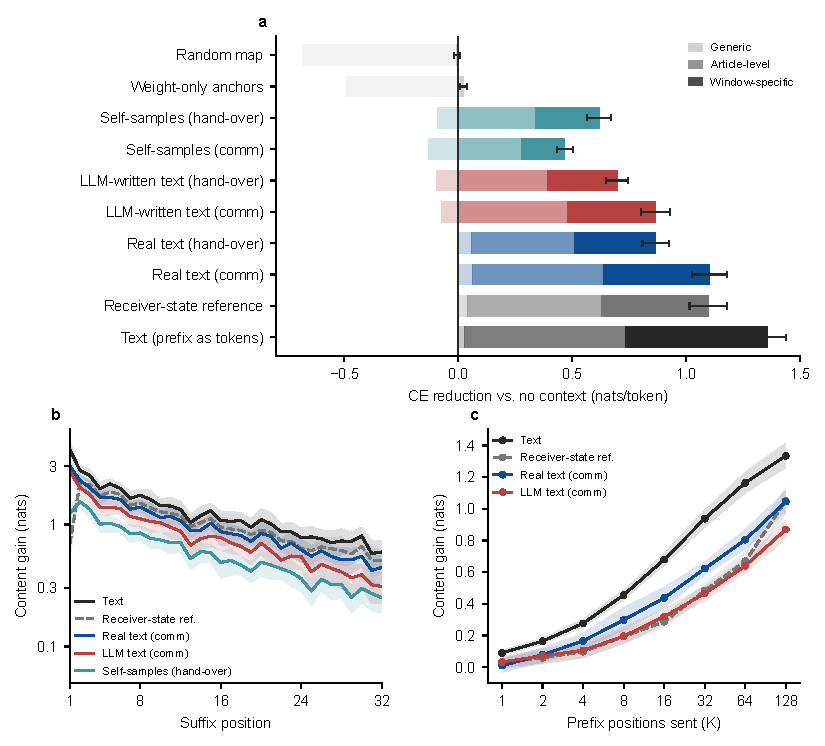
\includegraphics[width=\linewidth]{figs/fig_comm.pdf}
\caption{\textbf{What a latent message is worth to the receiver} (pythia-70m layer 2 $\to$ pythia-160m layer 1; $B$ sees only the 32-token suffix). \textbf{a}, Reduction in $B$'s suffix cross-entropy relative to no context on 493 test windows from 54 WikiText-103 articles (windows inside one article that have a same-article donor), decomposed with donor messages (\S\ref{sec:protocol}): generic (a message from another article), article-level (another window of the same article, minus another article) and window-specific (own window, minus a same-article window). Negative generic parts are drawn left of zero. Error bars: 95\% interval of the content part (article-level + window-specific) from a bootstrap over articles, fitting seeds and donor draws. \textbf{b}, Content gain at each suffix position (log scale) and \textbf{c}, when only the last $K$ prefix positions are sent (for text, $B$ reads the last $K$ prefix tokens); both use all 512 windows and one other-article donor per window, with pointwise 95\% article-bootstrap bands.}
\label{fig:comm}
\end{figure}

\subsection{Choosing where to bridge}
\label{sec:where}
The protocol fixes an injection depth $L_B$, and everything $B$ computes below it on the suffix is computed without the prefix. Injecting $B$'s own prefix states shows what this costs (Appendix~\ref{app:ceiling}): with pythia-160m as $B$, this reference reaches \CEILLONE\% next-token accuracy at $L_B=1$ but only \CEILLSIX\% at $L_B=6$, against \CEILFULL\% with the full prefix and \CEILNONE\% with none. Mid-depth hand-over, the usual stitching configuration, leaves little room for communication. We selected $(L_A, L_B)$ on the WikiText \emph{validation} split with a short real-text fit (Appendix~\ref{app:sweep}): $L_A=2$, $L_B=1$ minimised validation cross-entropy, with $L_A=1$--3 close behind. Mapping $A$'s final hidden state (after its output layer norm) gave the worst validation cross-entropy at both $L_B$ (4.64 and 4.55, against 4.03). \FREESWEEP

\subsection{A valid control needs donors from other documents}
\label{sec:generic}
Swapping messages between examples is the natural control for latent communication \citep[cf.][]{du2025interlat}, but which examples supply the swapped message matters. Our first analysis rolled messages within each batch of 16 windows. Because test windows are sorted by text position, 83\% of those donors came from the same article (427 of 512), and the control attributed 54\% of the real-text bridge's benefit (0.59 of 1.10 nats) to ``generic'' context. With donors drawn from other articles, the generic part of the same bridge is 0.06 nats [0.03, 0.10], or 6\% of its benefit (Figure~\ref{fig:comm}a). For text it is 0.03 nats [$-$0.00, 0.06] of a 1.36-nat benefit. Nearly all of the benefit of a real prefix or a real-text bridge is therefore content, and about half of that content is shared across windows of the same article (article-level 0.71 and window-specific 0.62 nats for text). A same-article donor removes that shared half along with the generic part. The decompositions below use donors from other articles and from the same article (five random draws of each per window, donors restricted to windows inside one article), evaluated on the 493 recipient windows that lie inside one article and have a same-article donor, so that generic, article-level and window-specific parts sum exactly to the total. Intervals come from a bootstrap that resamples articles, fitting seeds and donor draws.

\subsection{Bridges fitted on synthetic text deliver most of the receiver-state reference}
\label{sec:datafree}
Table~\ref{tab:comm} reports the decomposition for every message source. We compare against the \emph{receiver-state reference}, $B$'s own prefix states injected the same way. The reference is not an upper bound (a bridge could supply states that suit the spliced computation better), but it is a natural yardstick: it is what $B$ itself would have sent. We report two ratios: of content gains, which isolates what depends on the particular prefix, and of total gains, which also counts how the receiver fares with an irrelevant message.

\emph{A real-text bridge comes close to the reference.} With the communication objective, its content gain is 1.04 nats against the reference's 1.06, a ratio of 0.99 [0.94, 1.03] (per seed 0.94, 1.01, 1.01); its total gain is 1.00 [0.97, 1.04] of the reference's. A linear map from a 70M model's layer-2 states thus lets a 160M receiver predict the suffix about as well as its own layer-1 states would. Panel~b shows how the profile differs: at the first suffix position the bridged message is far more useful than the reference, while later positions fall slightly below it. One possible reason is that $A$'s layer-2 states have mixed in more of the prefix than $B$'s layer-1 states; we did not test this.

\emph{LLM-written text gets 82\% of the reference's content.} Fitted on 382k characters of encyclopedia-style text written by an LLM with no access to any corpus, the communication-objective bridge reaches a content gain of 0.86 nats: 0.82 [0.79, 0.85] of the reference (per seed 0.80, 0.81, 0.85) and 0.83 of the real-text bridge. Counting total gain, the ratio is lower, 0.72 [0.68, 0.76], because synthetic-text bridges have a \emph{negative} generic part: with a message about a different article, $B$ does worse on average than with no message at all ($-0.07$ nats [$-0.11$, $-0.04$] for LLM-written text, $-0.13$ for self-samples), whereas real-text bridges help slightly even then. Is this harm a general weakness of the receiver, or of the hidden-state interface? Neither: given an unrelated article's prefix \emph{as text}, $B$ does not get worse on average (generic part $+0.03$), and neither does it with an unrelated article's receiver-state reference ($+0.04$) or an unrelated message through the real-text bridge ($+0.06$). Paired per window against the text channel, the irrelevant-message effect differs by $+0.01$ [$-0.00$, 0.03] for the reference, $+0.03$ [0.02, 0.05] for the real-text bridge, but $-0.10$ [$-0.12$, $-0.08$] for the LLM-text bridge and $-0.16$ [$-0.17$, $-0.14$] for the self-sample bridge; averaged over seeds and donors, an irrelevant message worsens CE in 66\% and 81\% of windows for these two, against 48\% for irrelevant text (intervals from an article bootstrap, conditional on the saved fits and donor draws). For this pair and domain, the extra fragility is specific to bridges fitted on synthetic text. It is not universal: in other settings irrelevant messages also hurt through real-text bridges (generic part $-0.07$ with pythia-410m as receiver, $-0.02$ on reviews, $-0.35$ on code) and even as text ($-0.18$ with pythia-410m as receiver, $-0.26$ on code; Appendix~\ref{app:general}). Relative to the real-text bridge, the LLM-text bridge's shortfall of 0.31 nats splits into 0.17 [0.14, 0.21] of content and 0.13 [0.11, 0.16] of generic gain.

\emph{Self-samples and weight algebra fall far short.} Bridges fitted on samples from $A$ and $B$ themselves reach 0.44 [0.42, 0.47] of the reference's content with the communication objective and 0.59 [0.55, 0.62] with the hand-over objective. The best LLM-text bridge exceeds the best self-sample bridge by 0.25 nats [0.21, 0.28] of content; under matched objectives the margins are 0.40 [0.36, 0.44] (communication) and 0.08 [0.04, 0.11] (hand-over). The probe pools differ in more than their source (8.8M characters of real text; 382k characters, 88k tokens, of LLM text; 512 sampled sequences, 82k tokens, of self-samples), so these comparisons are between recipes, not between text sources at equal budget; \S\ref{sec:scale} compares real and LLM-written text at equal size. The weight-only least-squares map reaches a content gain of 0.02 nats [0.01, 0.04], 2\% of the reference, together with a generic loss of 0.49 nats. The random map shows no detectable content gain ($-0.01$ [$-0.02$, 0.01]).

\begin{table}[t]
\centering\small
\caption{Communication setting, pythia-70m L2 $\to$ pythia-160m L1, on 493 test windows (54 articles) that lie inside one article and have a same-article donor. Suffix CE in nats/token; gains relative to $B$ with no context (CE 4.930). Generic + content = total gain; the split of content into article-level and window-specific parts is shown in Figure~\ref{fig:comm}a. Content and net ratios divide a bridge's content and total gains by those of the receiver-state reference. 95\% intervals from a bootstrap over articles, fitting seeds and donor draws (4000 draws); fitted bridges average three seeds, all conditions average five donor draws of each kind.}
\label{tab:comm}
\resizebox{\linewidth}{!}{\footnotesize\setlength{\tabcolsep}{3pt}\begin{tabular}{lccccc}
\toprule
Message source (objective) & Total & Generic & Content & Content ratio & Net ratio \\
\midrule
Random map & $-$0.690 & $-$0.684 & $-$0.006 [$-$0.019, 0.007] & $-$0.01 [$-$0.02, 0.01] & $-$0.63 [$-$0.68, $-$0.59] \\
Weight-only anchors & $-$0.469 & $-$0.491 & 0.022 [0.005, 0.039] & 0.02 [0.00, 0.04] & $-$0.43 [$-$0.46, $-$0.40] \\
\midrule
Self-samples (hand-over) & 0.525 & $-$0.093 & 0.618 [0.566, 0.672] & 0.59 [0.55, 0.62] & 0.48 [0.45, 0.52] \\
Self-samples (comm) & 0.338 & $-$0.129 & 0.467 [0.434, 0.504] & 0.44 [0.42, 0.47] & 0.31 [0.29, 0.33] \\
LLM-written text (hand-over) & 0.601 & $-$0.096 & 0.697 [0.649, 0.746] & 0.66 [0.64, 0.68] & 0.55 [0.52, 0.57] \\
LLM-written text (comm) & 0.792 & $-$0.073 & 0.865 [0.803, 0.930] & 0.82 [0.79, 0.85] & 0.72 [0.68, 0.76] \\
Real text (hand-over) & 0.866 & 0.059 & 0.807 [0.750, 0.866] & 0.76 [0.74, 0.80] & 0.79 [0.76, 0.82] \\
Real text (comm) & 1.102 & 0.062 & 1.040 [0.963, 1.116] & 0.99 [0.94, 1.03] & 1.00 [0.97, 1.04] \\
\midrule
Receiver-state reference & 1.097 & 0.042 & 1.055 [0.974, 1.138] & 1 & 1 \\
Text (prefix as tokens) & 1.357 & 0.028 & 1.329 [1.247, 1.410] & 1.26 [1.23, 1.29] & 1.24 [1.21, 1.27] \\
\bottomrule
\end{tabular}
}
\end{table}

\subsection{Per transmitted position, the latent message is worth less than text}
\label{sec:bandwidth}
Hidden states are often assumed to carry more than the tokens they sit on. For this receiver and these bridges, that is not what we measure. At full length, the receiver-state reference delivers 79\% of the content gain that text delivers (1.06 vs 1.33 nats; Table~\ref{tab:comm}); one difference between the two is that with the message, $B$'s first layer processes the suffix without the prefix. When only the last $K$ prefix positions are sent (Figure~\ref{fig:comm}c), $K$ tokens of text are worth more than $K$ bridged positions at every tested $K\in\{1,2,4,\dots,128\}$: the difference between text and the real-text bridge ranges from 0.08 nats [0.04, 0.12] at $K=1$ to 0.36 [0.30, 0.43] at $K=64$, and all eight Bonferroni-adjusted intervals exclude zero (smallest lower bound 0.02; intervals resample articles and are conditional on the saved bridges and one other-article donor draw). This is an operational result for this receiver, not a statement about information density. Short messages also change other things: the bridges were fitted only on 128-position messages, a truncated message places a mid-document state at sequence position 0, and absolute cross-entropy with a short latent message is \emph{worse} than with no context (Appendix~\ref{app:bandwidth}). Bridges trained for short messages, or receivers that inject at several layers or into key--value caches \citep{fu2026c2c}, may behave differently.

Equal numbers of positions are not equal communication costs. Payload: a 128-position message costs 262\,kB in float32 if $A$'s 512-dimensional states are sent and the bridge is applied at the receiver (131\,kB in float16), or 393\,kB if the bridged 768-dimensional states are sent; 128 token ids packed as 16-bit integers cost 256 bytes, so the latent message is about three orders of magnitude larger. Computation: in an idealised split implementation the receiver still runs 11 of its 12 layers on every message position, roughly the same as reading the prefix as text (a dense-layer estimate of $2\times85$M non-embedding parameters $\times128$ positions $\approx 22$ GFLOP either way), and the sender adds two of its layers; our implementation runs both models in full and overwrites states, so it does not realise even that. We did not measure latency. This design therefore shows no communication-efficiency advantage; the case for latent channels rests on settings where the sender would otherwise have to \emph{generate} text token by token, the motivation of \citet{fu2026c2c} and \citet{zou2025latentmas}, which we do not test.


\subsection{How far the findings generalise}
\label{sec:scale}

Table~\ref{tab:general} repeats the measurement across model pairs, model families and test domains. The content contrast can grow because matched messages help more or because irrelevant messages hurt more, so for each bridge we report both its content ratio and its \emph{net} ratio: the total reduction in cross-entropy relative to no context, divided by the reference's. Appendix~\ref{app:general} lists the populations and protocol differences.

\begin{table}[t]
\centering\small
\caption{Generalisation. For each bridge, content gain (other-document donor minus matched message) and net gain (no context minus matched message), each relative to the receiver-state reference of the same receiver on the same windows; reference content in nats. 95\% intervals over documents, fitting seeds and donor draws. All bridges use the communication objective; layer pairs were selected on validation text for each model pair. The code and review rows evaluate the main pair's bridges, fitted on WikiText-like text, without refitting. Too few review windows have a same-document donor to split content into article-level and window-specific parts (Appendix~\ref{app:general}).}
\label{tab:general}
{\footnotesize\setlength{\tabcolsep}{4pt}\input{tab_general}}
\end{table}

\paragraph{The receiver's own states are matched only in some pairs.} In-domain, the real-text bridge's net ratio is close to 1 when pythia-70m, pythia-410m or GPT-2 sends to pythia-160m (1.00, 0.99 and 1.00). It is lower, 0.87 [0.82, 0.92], when pythia-160m sends to pythia-410m, a receiver whose own states are far more useful (1.51 nats of content, 93\% of what text gives it). The shortfall could come from the sender, the bridge's capacity or optimisation, or the restricted layer search, since the selected sender layer was the deepest candidate; we cannot tell these apart. The main pair shows that a less capable sender is not by itself an obstacle.

\paragraph{No net improvement was detected with a stronger sender.} We replaced pythia-70m by pythia-410m as sender to the same receiver, on identical windows and donors. The LLM-text bridge's content ratio rises from 0.82 to 0.89, but the net gain does not change detectably for any probe source, and its point estimates are slightly lower. For real text, LLM text and self-samples, the net gain changes by $-0.01$ [$-0.06$, 0.04], $-0.03$ [$-0.07$, 0.01] and $-0.00$ [$-0.09$, 0.11] nats, and the content gain by $+0.03$ [$-0.03$, 0.11], $+0.07$ [0.04, 0.11] and $+0.11$ [$-0.01$, 0.22]. The bootstrap pairs fitting seeds across senders, which share probe and minibatch seeds, and uses identical donor draws. Only the LLM-text bridge's content change is detectably positive, and in these fits its larger contrast reflects worse predictions with irrelevant messages rather than better ones with relevant messages. Read alone, the content contrast would suggest an improvement that the net gain does not show.

\paragraph{Other model families.} \XFAMILYRESULTS

\paragraph{Other domains.} The main pair's bridges were fitted for encyclopedia-like text. On long IMDB reviews (at least 322 tokens, 30\% of the test split), the domain's own reference is weaker, with 0.43 nats of content, and the bridges keep most of its content and net gain. Their content and net ratios are 0.81 and 0.71 for real text, 0.73 and 0.63 for LLM text, and 0.46 and 0.46 for self-samples.

On Python source code, all three retain about 30\% of the reference's content, but their net effects diverge. The self-sample bridge still helps (net ratio 0.21 [0.19, 0.24]), the real-text bridge's effect is unresolved (0.03 [$-0.03$, 0.10]), and the LLM-text bridge leaves the receiver worse off than no message ($-0.10$ [$-0.16$, $-0.03$]). On code, even an unrelated file's prefix given as text hurts the receiver (generic part $-0.26$). Relative performance falls sharply on this corpus, and which bridge is useful there is not predicted by which is best in-domain.

\paragraph{Text source and amount.} \TEXTSOURCES

\paragraph{Bridge capacity.} \CAPACITY

\subsection{Hand-over stitching answers a different question}
\label{sec:diag}
In the classical hand-over setting, $B$ reads the tokens, but the bridged $A$ state replaces every layer-$L_B$ state. Bridged systems score below $A$ alone on accuracy, both here and on two small testbeds (Appendix~\ref{app:small}). Table~\ref{tab:diag} varies optimisation length, bridge capacity and layer pairing for 70M$\to$160M. It uses a real-text probe, one seed and 512 test windows. We interpret this diagnostic descriptively because it uses a single seed and checkpoints chosen post hoc.

\begin{table}[h]
\centering\small
\caption{Hand-over setting, pythia-70m $\to$ pythia-160m: next-token accuracy (\%) / cross-entropy (nats) over all 128 positions; one seed. $A$ alone: 25.65 / 4.626; $B$ alone: 30.60 / 4.074. Bridges start from the weight-only map and are trained with Adam at a constant learning rate of $10^{-3}$; the 1500- and 3000-step entries are checkpoints of the same run.}
\label{tab:diag}
\begin{tabular}{lccc}
\toprule
& 600 steps & 1500 steps & 3000 steps \\
\midrule
L3$\to$L6, linear & 21.67 / 4.785 & 23.61 / 4.615 & 22.69 / 4.706 \\
L3$\to$L6, linear + MLP (2048) & 22.38 / 4.710 & 23.82 / 4.582 & 24.64 / 4.535 \\
\midrule
\multicolumn{4}{l}{Depth-matched pairs, linear, 600 steps:} \\
\quad L1$\to$L2 / L2$\to$L4 & \multicolumn{3}{c}{22.44 / 4.786 \qquad 19.71 / 4.998} \\
\quad L4$\to$L8 / L5$\to$L10 & \multicolumn{3}{c}{23.00 / 4.712 \qquad 23.40 / 4.702} \\
\quad L6 (final, after the output layer norm)$\to$L12 & \multicolumn{3}{c}{13.70 / 6.178} \\
\bottomrule
\end{tabular}
\end{table}

No configuration reaches $B$ alone, and none exceeds $A$'s accuracy. The longest-trained non-linear bridge nevertheless has \emph{lower} cross-entropy than $A$ alone, at 4.535 against 4.626. Whether a stitched system ``performs worse than the sender'' therefore depends on the metric and on training, and this observation does not establish a bound: in principle, a downstream decoder can use a representation better than the sender's own upper layers do.

Training length and capacity matter too. At 3000 steps, the non-linear bridge closes 75\% of the accuracy gap between the 600-step linear bridge and $A$ alone. With a constant learning rate, the linear map's accuracy is not monotone in training length: 23.61 at 1500 steps and 22.69 at 3000. Comparisons between stitches based on single checkpoints therefore require caution.

$A$'s final hidden state, taken after its output layer norm, is a poor source both here and in the communication setting (\S\ref{sec:where}). We did not test the pre-normalisation final residual state, so these results say nothing about the information present before $A$'s last normalisation.

In the communication setting, $B$ keeps its own suffix computation and receives only what it lacks. We ask whether the message improves $B$ beyond the benefit of any message. Comparing the stitched system with either model answers a different question.



\section{Discussion}
\label{sec:discussion}

\paragraph{Evaluating latent channels.}
The donor control is cheap, one extra forward pass per donor message, and the choice of donor changes the conclusion. With donors from other documents, nearly all of the benefit of text, of the receiver's own states and of real-text bridges in the main pair is content; with donors from the same document, about half of that content is silently counted as generic. Work that contrasts matched with swapped messages, for training \citep{du2025interlat} or evaluation, should state where the swapped messages come from. We also recommend reporting the receiver's own states injected the same way. In our setting this reference shows how quickly the benefit of a message falls with injection depth, and that even at the shallowest depth it delivers less content than the corresponding text.

\paragraph{Building bridges without real corpus text.}
An LLM that wrote encyclopedia-style text without access to any corpus supplied probe text good enough for a bridge that delivers 82\% of the receiver-state reference's content. The models' own samples and weight algebra are much weaker substitutes. In the main WikiText experiment, the tested synthetic fitting recipes cost more than content: with these bridges a message about a different document leaves the receiver worse off on average than no message at all, while the real-text bridge and plain text do not. In other settings real-text bridges and plain text can also be hurt by irrelevant messages, and on reviews the self-sample bridge's generic part is not negative (\S\ref{sec:scale}); we compare complete recipes and do not isolate synthetic provenance as the cause. For systems that may receive irrelevant messages this is a robustness cost that a no-context comparison hides; behaviour under adversarially chosen messages remains untested. We do not know whether a small amount of in-domain text would remove it; testing that directly is an obvious next step. \SCALEDISCUSSION

\paragraph{Relation to weight-space reasoning.}
The study began from evidence that frontier models can read and edit network weights \citep{takehi2026sparks}. In small testbeds an LLM designed complete bridges from weights alone (Appendix~\ref{app:small}). At pretrained-model scale its useful contribution narrowed to supplying in-register text, and the distribution-matching recipe it had proposed on the small testbed; our experiments do not separate the LLM's world knowledge from register and topic coverage as the reason the text works. The weight-only map we tested, a least-squares fit between embedding matrices in the spirit of the within-model alignment of LatentMAS \citep{zou2025latentmas}, delivered 2\% of the reference. This rules out that particular map, not weight-based alignment in general.

\section{Limitations}
\label{sec:limitations}
\begin{itemize}
\item \textbf{Scale and family.} \XFAMILYLIMIT
\item \textbf{One task, few domains.} We measure next-token prediction, fitted on WikiText-like text and tested on WikiText, long movie reviews and Python code. We do not test whether the measured content predicts benefits in downstream collaboration such as question answering or reasoning.
\item \textbf{Cross-family protocol.} Cross-family pairs use a sender message length chosen from the test inputs, so the sender often reads less of the prefix than the receiver-state reference (93\% of its tokens for GPT-2 into Pythia, 74\% into Qwen2.5), and we have no position-matched no-context control for receivers with absolute positions. Their results are protocol-specific case studies. Two further planned pairs were dropped for compute after the first cross-family run had started (Appendix~\ref{app:general}), so the three reported pairs are not a blind or representative sample, and their intervals do not include pair-selection uncertainty.
\item \textbf{One receiver design.} The receiver gets a single residual-stream injection at one layer. Multi-layer or key--value injection may raise what latent messages can deliver, and the text-versus-latent comparison is specific to this design.
\item \textbf{Synthetic corpora.} Main results use one LLM, one prompt and 64 topic areas; the variant experiment adds one corpus from a second LLM and one fiction corpus, each a single generated sample that also differs in token count and topic coverage. The second LLM was run through an agentic command-line tool in a read-only sandbox, which restricts but does not remove tool access; we did not pin its model version. We cannot rule out that either LLM's pretraining included WikiText-like text.
\item \textbf{Log-score, not information.} Gains are differences in expected log-score through a fixed receiver. They measure usefulness to that receiver, not the mutual information between message and prefix.
\item \textbf{Statistics.} Intervals resample test articles, fitting seeds and donor draws, but with only two or three fits per condition the seed component is poorly estimated, and the donor pool itself is fixed (donors are other test windows). Per-seed values are reported for the main pair. Diagnostics (\S\ref{sec:diag}) and layer sweeps use one seed. \SCALESEEDS
\end{itemize}


\section*{Use of AI tools}
The experiments were designed, implemented and run with an AI coding assistant (Claude, Anthropic) under the author's direction. The manuscript was also drafted with this assistant under the author's direction. A second model (GPT, OpenAI) then audited the manuscript and code in repeated rounds through the Codex command-line tool with read-only access. It recomputed the reported numbers from the retained per-window arrays. These audits were model-assisted checks and did not constitute independent replication. The models also generated the encyclopedia-style probe text used to fit the synthetic-text bridges (\S\ref{sec:method}). The author takes full responsibility for the content.

\bibliographystyle{plainnat}
\bibliography{refs}

\appendix
\section{Receiver-state reference versus injection depth}
\label{app:ceiling}
We inject $B$'s own layer-$L_B$ prefix states, computed with $B$ reading the prefix alone, into $B$'s suffix pass at the same layer (128 test windows; a diagnostic, not used for any selection; script \texttt{pb\_ceiling.py}, output \texttt{ceiling.txt}).

\begin{table}[h]
\centering\small
\begin{tabular}{lcccccc}
\toprule
Injection layer $L_B$ & 1 & 2 & 3 & 4 & 6 & 8 \\
\midrule
pythia-160m as $B$: accuracy (\%) & 34.3 & 33.4 & 32.4 & 31.4 & 26.2 & 25.0 \\
pythia-70m as $B$: accuracy (\%) & 28.5 & 27.8 & 25.4 & 20.4 & -- & -- \\
\bottomrule
\end{tabular}
\caption{References on the same windows: pythia-160m with the full prefix 37.1\%, with none 24.0\%; pythia-70m 31.9\% and 19.8\%. Below the injection layer $B$ processes the suffix without the prefix, and the benefit of its own prefix states falls quickly with depth.}
\end{table}

\section{Layer selection on the validation split}
\label{app:sweep}
For each $(L_A, L_B)$ we fit a linear bridge on real text with the communication objective (300 steps, seed 0) and score its suffix cross-entropy on 256 non-overlapping WikiText-103 \emph{validation} windows. Selection uses this matched cross-entropy only.

\begin{table}[h]
\centering\small
\begin{tabular}{lcccccc}
\toprule
$L_A$ (pythia-70m) & 1 & 2 & 3 & 4 & 5 & 6 (final, post-LN) \\
\midrule
$L_B=1$ & 4.235 & \textbf{4.031} & 4.106 & 4.195 & 4.126 & 4.641 \\
$L_B=2$ & 4.083 & 4.086 & 4.103 & 4.176 & 4.187 & 4.555 \\
\bottomrule
\end{tabular}
\caption{Validation suffix CE (nats/token). Receiver-state reference on the same windows: 3.908 ($L_B=1$), 3.969 ($L_B=2$).}
\end{table}

\SWEEPAPPENDIX

\section{Truncated messages: absolute cross-entropy}
\label{app:bandwidth}
Suffix CE (nats/token) when only the last $K$ prefix positions are sent; fitted bridges are the mean of three seeds. $B$ with no context: 4.924.

\begin{table}[h]
\centering\small
\resizebox{\linewidth}{!}{%
\begin{tabular}{lcccccccc}
\toprule
$K$ & 1 & 2 & 4 & 8 & 16 & 32 & 64 & 128 \\
\midrule
Text (last $K$ tokens) & 4.822 & 4.747 & 4.627 & 4.447 & 4.221 & 3.978 & 3.746 & 3.572 \\
Receiver-state reference & 5.127 & 5.151 & 5.115 & 4.970 & 4.785 & 4.527 & 4.266 & 3.836 \\
Real-text bridge (comm) & 5.233 & 5.294 & 5.286 & 5.200 & 5.004 & 4.717 & 4.434 & 3.827 \\
LLM-text bridge (comm) & 5.205 & 5.320 & 5.390 & 5.369 & 5.258 & 5.080 & 4.871 & 4.137 \\
\bottomrule
\end{tabular}}
\caption{Short latent messages are worse than no context in absolute terms, including $B$'s own states (reference, $K\le 8$). A message of $K<P$ positions places a mid-document state at sequence position 0, where Pythia normally sees the start of a text, and the bridges were fitted only with 128-position messages. We have not isolated which of these causes the drop, and the content contrasts in Figure~\ref{fig:comm}c, which compare matched and other-article messages of the same length, may also be affected.}
\end{table}

\section{Generalisation experiments: populations and protocol differences}
\label{app:general}

\paragraph{Populations.} Pythia and cross-family rows of Table~\ref{tab:general} with pythia-160m as receiver use the main pair's 493 windows from 54 articles; the pythia-410m receiver uses the same windows. GPT-2$\to$Qwen2.5 and OPT$\to$GPT-2 define windows in their receivers' tokenisations; after the same restrictions each analyses 484 windows from 53 articles. Domain windows are listed in \texttt{dom\_code\_windows.json} and \texttt{dom\_reviews\_windows.json} (directory \texttt{out\_pb}), a retrospective reconstruction from the same inputs and selection rules whose document identities match the saved runs (the original runs did not store offsets). \emph{Code}: top-level Python standard-library files with at least two non-overlapping 161-token windows; up to four windows per file were drawn and 512 sampled from them (157 files); the decomposition uses the 509 windows from 154 files that have a same-file donor. \emph{Reviews}: IMDB test reviews with at least 322 Pythia tokens (7{,}440 of 25{,}000, i.e.\ long reviews only); 512 windows from 501 reviews. Only 22 windows have a same-review donor, so for reviews we estimate generic and content parts on all 512 windows and do not split content into article-level and window-specific parts. Donors in both domains come from other documents, with five random draws per window. Intervals resample documents, fitting seeds and donor draws, and are conditional on the selected documents and the fixed donor pool.

\paragraph{Irrelevant messages beyond the main pair.} Generic parts (no context minus other-document donor, nats): pythia-160m$\to$pythia-410m, real-text bridge $-0.07$ [$-0.12$, $-0.02$], text $-0.18$ [$-0.23$, $-0.13$]; reviews, real-text bridge $-0.02$ [$-0.04$, $-0.00$], text $+0.04$; code, real-text bridge $-0.35$ [$-0.38$, $-0.32$], text $-0.26$ [$-0.29$, $-0.24$].

\paragraph{Cross-family protocol.} Five cross-family pairs were planned. We reduced the suite about half an hour after the first run, GPT-2 into Pythia, had started. Some results may already have been printed. To fit the compute budget, we dropped Pythia-160M into SmolLM2-135M and Pythia-160M into GPT-2. We also dropped self-sample probes for GPT-2 into Qwen2.5 and OPT into GPT-2 (\texttt{out\_pb/x\_skip.txt}, \texttt{x\_lean.txt}). None of the dropped fits was run, but the choice of reported pairs was not blind. Windows and targets are defined in the receiver's tokenisation ($P_B=128$ prefix and $S=32$ suffix tokens). The sender receives the decoded prefix text, re-tokenised with its own tokenizer and truncated to its last $P_A$ tokens so that every message has the same length. $P_A$ is the shortest re-tokenised prefix among the test windows ($P_A=118$ for GPT-2 into Pythia; prefix lengths range from 118 to 151, median 127). This choice uses test inputs but no targets; it truncates 511 of 512 prefixes and keeps on average 93\% of the sender's prefix tokens, while the receiver-state reference uses all 128 receiver-token states. For GPT-2 into Qwen2.5, $P_A=90$ (prefix lengths 90 to 146, median 123; prefix length correlates at $-0.85$ with the share of digits, which Qwen tokenises one per token), so the sender keeps on average only 74\% of its prefix tokens. Probe and validation windows whose sender prefix is shorter than $P_A$ are dropped. For the real-text and LLM-written probes, 4029 to 4094 of 4096 windows are kept per pair and seed, and 253 to 256 of 256 validation windows (listed in \texttt{out\_pb/general\_audit.json}). The GPT-2$\to$Pythia self-sample probes (two seeds) were generated in memory and not saved, so their filtering counts are not available. Suffix states are computed with position ids that start at the message length. For receivers with absolute position embeddings (GPT-2 as receiver), the no-context control starts at position 0, so generic and net parts may include a position-offset effect; content contrasts compare matched and donor messages at identical positions. The weight-only map is fitted on tokens whose strings occur in both vocabularies. The cross-family runner forms self-sample probe text by concatenating decoded samples and drawing windows from it, unlike the Pythia runner, which uses the generated sequences directly.

\paragraph{Text variants.} The variant corpora were concatenated in file order and truncated to 371{,}254 characters each, which keeps 22 complete encyclopedia articles from the first LLM (85k Pythia tokens), 20 from the second (72k tokens) and all 24 fiction texts (96k tokens). Four fiction generations were interrupted when the machine slept and were regenerated with the same prompt; only the final files are archived.


\section{Reproducibility}
\label{app:repro}
\textbf{Data.} WikiText-103 raw \citep{merity2016wikitext}: the first 30{,}000 training lines (8.8M characters) form the real-text pool; the first 6{,}000 test lines give 512 non-overlapping 161-token test windows (seed 123); the first 6{,}000 validation lines give 256 windows for layer selection. \textbf{LLM-written text.} Each article was requested with the prompt ``Write about 2,500 words of original encyclopedia articles in the plain, factual style of Wikipedia, with section headings written like `= = History = ='. Topic area: \emph{X} (invent plausible specifics freely; do not copy any real article). Output only the article text.'' using Claude Opus 5.5 at low effort with all tools disabled, an empty working directory and no session persistence. Of 20{,}604 non-overlapping 50-character windows of the 1.03M-character collection, 2 occur verbatim in the test text and 1 in the validation text; all three are stock phrases (e.g.\ ``\ldots by the Recording Industry Association of Amer[ica]''). \textbf{Self-samples.} 512 sequences, 128 each from two seeds of $A$ and of $B$, unconditional from the end-of-text token at temperature 1. \textbf{Compute.} One Apple M5 Pro (Metal backend, float32). A 600-step fit of the 70M$\to$160M bridge together with its evaluation took 4--6 minutes when run alone. Timing ledger (process time, several processes sharing one GPU): the timed fits in the logs of the main, generalisation and diagnostic runs (\texttt{out\_pb/*.log}) total 22.8 hours, and the earlier Pythia seed runs (\texttt{out\_pythia/seeds.log}) 1.1 hours; layer sweeps and donor evaluations were not timed, and the timed parts of aborted runs are excluded. The main and generalisation suite ran from 3 November 12:30 (first log) to 4 November 04:58 GMT (last result file), 16.5 hours of wall-clock time; the earlier Pythia runs and later audit scripts fall outside this interval. \textbf{Code.} Scripts, logs, per-window results, fitted bridges, probe texts, pinned environments (\texttt{requirements-lock.txt}), the Hugging Face revisions of every model and dataset (enforced in the loaders) and a manifest of full SHA-256 file hashes are kept together, with the run scripts actually used (\texttt{out\_pb/queue*.sh}). The archive supports numerical reanalysis of every reported result; reconstruction of the experiments is documented for the main \texttt{pb*} suite, whereas the small-testbed harness of Appendix~\ref{app:small} needs a sandbox set-up that is only partly documented. Model and dataset revisions are pinned in all retained loaders. The archive is released at \url{https://github.com/dongzhaohe321418-lab/content-or-context}. Not kept: transcripts of the second LLM's generations, failed fiction generations that were overwritten when regenerated, and all self-sample probe text (main, larger-Pythia and cross-family runs), which was generated in memory; the resulting bridges and evaluation arrays are kept. Probe windows are drawn with a sampler that never selects the last legal start position of the probe text; we kept it unchanged so that saved windows reproduce.

\section{Small-scale studies: an LLM designs the whole bridge from weights}
\label{app:small}

Before the Pythia study we ran two controlled testbeds in which the LLM (Claude Opus 5.5) designs the \emph{entire} bridge, not only the probe text, from the two models' weights. These results motivated the KL-matching recipe used in the main text, which the LLM itself proposed in the second testbed.

\paragraph{Conditions.} (i) \emph{Tool-free}: one turn, the weights printed as text, no code execution. (ii) \emph{Weight algebra only}: the model submits one Python program per turn, executed in a macOS \texttt{sandbox-exec} jail (no network, no read access to the workspace), and may not construct any input or run either network. (iii) \emph{Code and self-made probes}: as (ii), but it may synthesise inputs. In no condition does it see any training or test data. Every turn was logged and audited.

\paragraph{Digit classifiers.} Three pairs of two-hidden-layer MLPs trained on sklearn's $8\times8$ digits from different seeds: same width (16-16 and 16-16, ReLU); different width (16-16 and 24-24, ReLU); different width and activation (16-16 ReLU and 24-16 tanh). The bridge maps $A$'s first hidden layer to $B$'s first pre-activation; the score is $B$'s accuracy on 594 held-out images (95\% Wilson half-widths are about 1.5--2 points near 95\% accuracy and about 4 points near 50\%).

\begin{table}[h]
\centering\small
\resizebox{\linewidth}{!}{%
\begin{tabular}{lccc}
\toprule
Method & same & width & hetero \\
\midrule
$A$ alone / $B$ alone & 96.0 / 96.0 & 96.5 / 97.5 & 96.0 / 96.5 \\
Random bridge & 10.0 & 10.5 & 8.5 \\
Unit matching (Re-Basin style, data-free) & 32.3 & 33.8 & 40.1 \\
Weight-space least squares (data-free algorithm) & 84.3 & 89.9 & 90.1 \\
Best noise probe (selected on test; favours the baseline) & 88.0 & 93.6 & 89.1 \\
LLM, tool-free (3 runs: mean [min--max]) & 43.4 [20--82] & 63.2 [47--82] & 39.4 [10--73] \\
LLM, weight algebra only (1 run) & 83.3 & 95.3 & 87.7 \\
\textbf{LLM, code + self-made probes (2 runs)} & \textbf{94.9} & \textbf{94.9} & \textbf{93.9} \\
Fitted on real training images (upper reference) & 95.3 & 96.8 & 94.1 \\
\bottomrule
\end{tabular}}
\caption{Digit classifiers. With code, the LLM synthesised digits from stroke templates and fitted the bridge on them; pool sizes and augmentation differed between runs (per-run transcripts are archived). It exceeds the best noise probe by 1.3--6.9 points; we did not save per-image predictions, so we report no paired significance test, and the smallest difference (different-width pair, +1.3) should be treated as unresolved. Without tools it derives the right principle, $W_1^A M \approx W_1^B$, but cannot invert matrices by hand, hence the 10--82\% spread.}
\label{tab:digits}
\end{table}

\paragraph{Character-level GPTs.} Two 4-layer character-level transformers trained from different seeds on Python standard-library source, widths 64 and 96; the bridge connects their residual streams after layer 2 and the score is $B$'s next-character accuracy. $A$ alone scores 62.8 and $B$ alone 63.6. A bridge fitted on real code by minimising $B$'s next-character cross-entropy against the true characters reaches 55.58 (three seeds, s.d.\ 0.11). In condition (iii), the LLM started from the weights alone and implemented the forward pass from a textual specification. It derived a backward pass and checked it against numerical gradients. It then fitted the bridge on probe text it wrote itself and text sampled from $A$ and $B$. The two runs used different objectives: run 0 matched $B$'s own predictive distribution, run 1 matched an equal mixture of $A$'s and $B$'s distributions. They reached 55.0 and 55.7. Fitting the hard-target objective on text sampled from $A$ and $B$, with no LLM involved, reaches 54.95 (s.d.\ 0.06). These recipes are not algorithm-matched, so the comparison shows that self-sampling suffices on this testbed, not that the LLM's recipe is uniquely good. Python probe text written by the LLM without tools (52k characters from four calls) reaches 49.80 (s.d.\ 0.09), against 26.88 for the same characters shuffled. Two of the four calls returned a refusal and a meta-response instead of code, and we did not filter them, so 4.6\% of that probe file is not code. Of its non-overlapping 50-character windows, 1.1\% and 0.9\% (the two code-bearing calls) occur verbatim in the standard-library corpus from which the models' training split is taken (0.9\% and 0.9\% in the training split itself).

\paragraph{Two observations carried into the main study.} First, in the hand-over setting the bridged system scores below $A$ alone in accuracy on both language testbeds (55.7 vs 62.8 here; 21.1 vs 25.7 on Pythia). Section~\ref{sec:diag} shows that this gap depends on training length, capacity and metric, so it should not be read as information loss. Second, self-sampling is sufficient for tiny models trained on a narrow corpus, which raises the question of whether it remains sufficient for pretrained models with broad distributions. Section~\ref{sec:results} answers both.

\paragraph{A note on refusals.} One of the four archived calls asking the LLM to write probe programs for ``calibrating a connection between two models'' declined, reading the request as a covert-channel or steganography exercise; another returned a meta-response without code. The encyclopedia-article calls used a neutral description of the task (Appendix~\ref{app:repro}). We archived 64 outputs. Two numbered files from the first batches are missing, for reasons we did not record.


\end{document}
